The general strategy of the tmLQCD package is to provide programs for
the main applications used in lattice QCD with Wilson twisted mass
fermions. The code and the algorithms are designed to be general
enough such as to compile and run efficiently on any modern computer 
architecture. This is achieved code-wise by using standard C as
programming language and for parallelisation the message passing
interface (MPI) standard version 1.1.

Performance improvements are achieved by providing dedicated code for
certain widely used architectures, like PC's or the Blue Gene family. 
Dedicated code is mainly available for the kernel routine -- the
application of the Dirac operator, which will be discussed in
detail in section~\ref{sec:dirac}, and for the communication
routines.

The tmLQCD package provides three main applications. The first is an
implementation of the (P)HMC algorithm, the second and the third are
executables to invert the Wilson twisted mass Dirac operator
(\ref{eq:Dtm}) and the non-degenerate Wilson twisted mass Dirac operator
(\ref{eq:Dh}), respectively. All three do have a wide range of
run-time options, which can be influenced using an input file. The
syntax of the input file is explained in the documentation which ships
with the source code. The relevant input parameters will be mentioned
in the following where appropriate, to ease usage.

We shall firstly discuss the general layout of the three
aforementioned applications, followed by a general discussion of the
parallelisation strategy used in all three of them.

\subsection{{\ttfamily hmc\_tm}}

\begin{figure}[t]
  \centering
  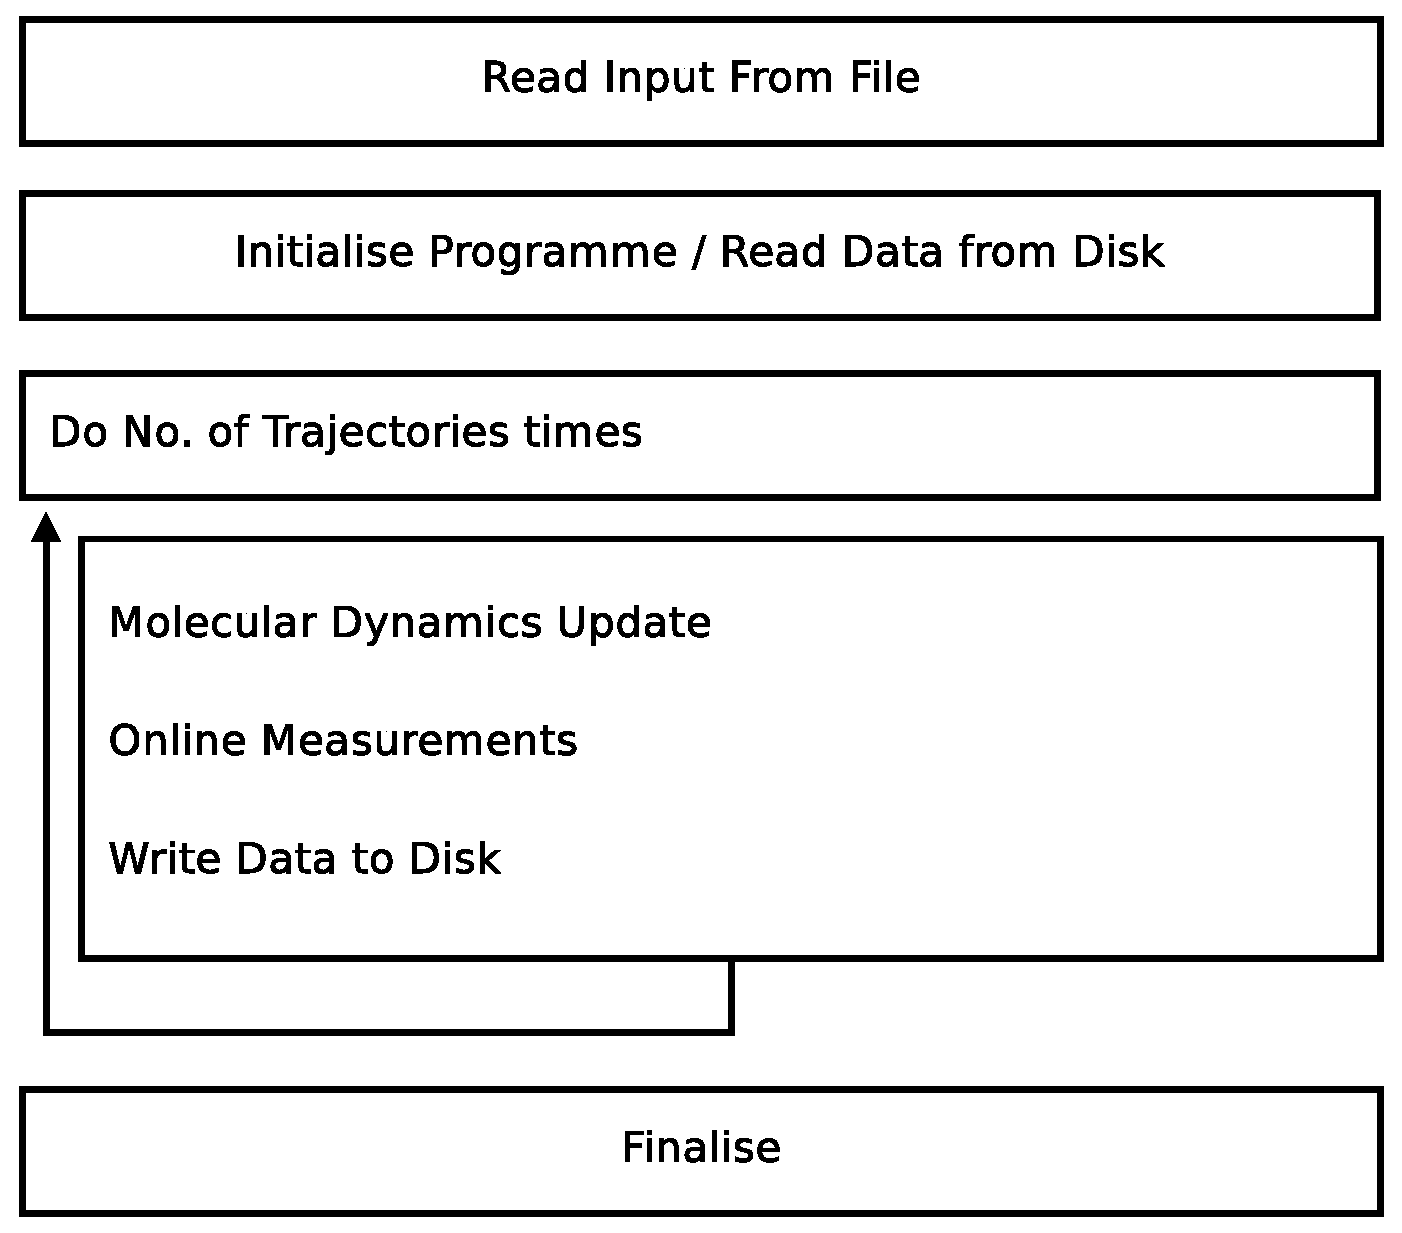
\includegraphics[width=0.7\linewidth]{hmcflow.eps}
  \caption{Flowchart for the {\ttfamily hmc\_tm} executable}
  \label{fig:hmcflow}
\end{figure}

In figure~\ref{fig:hmcflow} the programme flow of the {\ttfamily
  hmc\_tm} executable is depicted. In the first block the input file
is parsed and parameters are set accordingly. Then the required memory
is allocated and, depending on the input parameters, data is read from
disk in order to continue a previous run. 

The main part of this application is the molecular dynamics
update. For a number of trajectories, which must be specified in the
input file, first a heat-bath is performed, then the integration
according to the equations of motion using the integrator as specified
in the input file, and finally the acceptance step. 

After each trajectory certain online measurements are performed,
such as measuring the plaquette value. Other online measurements are
optional, like measuring the pseudo scalar correlation function. 

\subsubsection{command line arguments}

The programme offers command line options as follows:
\begin{itemize}
\item {\ttfamily -h|?} prints a help message and exits.
\item {\ttfamily -f} input file name. The default is {\ttfamily
    hmc.input}
\item {\ttfamily -o} the prefix of the output filenames. The default is
  {\ttfamily output}. The code will generate or append to two files,
  {\ttfamily output.data} and {\ttfamily output.para}.
\end{itemize}

\subsubsection{Input / Output}

The parameters of each run are read from an input file with default
name {\ttfamily hmc.input}. If it is missing all parameters will be
set to their default values. Any parameter not set in the input file
will also be set to its default value.

During the run the {\ttfamily hmc\_tm} program will generate two
output files, one called per default {\ttfamily output.data}, the
other one {\ttfamily output.para}. Into the latter important
parameters will be written at the beginning of the run.

The file {\ttfamily output.data} has several columns with the
following meanings
\begin{enumerate}
\item Plaquette value.
\item $\Delta H$
\item $\exp(-\Delta H)$
\item number of pseudo fermion monomials times two integers. The first
  of the two is the sum of solver iterations needed
  in the acceptance and heatbath steps, the second is the sum of 
  iterations needed for the force computation of the whole trajectory.
\item Acceptance ($0$ or $1$).
\item Time in seconds needed for this trajectory.
\item Value of the rectangle part in the gauge action, if used.
\end{enumerate}
Every new run will append its numbers to an already existing file.

In addition, the program will create a file {\ttfamily
  history\_hmc\_tm}. This file provides a mapping between the
configuration number and its plaquette and Polyakov loop
values. Moreover the simulation parameters are stored there and in
case of a reread the time point can be found there.

After every trajectory the program will save the current configuration
in the file {\ttfamily conf.save}.

At the end of each trajectory, the program edits the file {\ttfamily nstore\_counter} in the working directory.
This file contains one line with $3$ space-separated values: {\ttfamily i j confname}.
\begin{itemize}
  \item
  {\ttfamily i} is the index of the next gauge configuration that will be saved.
  \item
  {\ttfamily j} is the trajectory index of the latter.
  \item
  {\ttfamily confname} is the configuration name from which the HMC starts.
  If the {\ttfamily Startcondition} parameter is set to {\ttfamily hot} or {\ttfamily cold},
  the file is created or overwritten with the following content at each trajectory
  \footnote{The trajectory index starts from $0$, but the $0$-th trajectory is not saved.}: 
  %
  \begin{enumerate}
    \item 
    {\ttfamily 0 1 conf.save}
    \item 
    {\ttfamily 1 2 conf.0000}
    \item
    {\ttfamily 2 3 conf.0001}
    \item
    ... (and so on depending on the value of {\ttfamily Measurements} in the input file)
  \end{enumerate}
  %
\end{itemize}

\subsection{{\ttfamily invert} and {\ttfamily invert\_doublet}}

\begin{figure}[t]
  \centering
  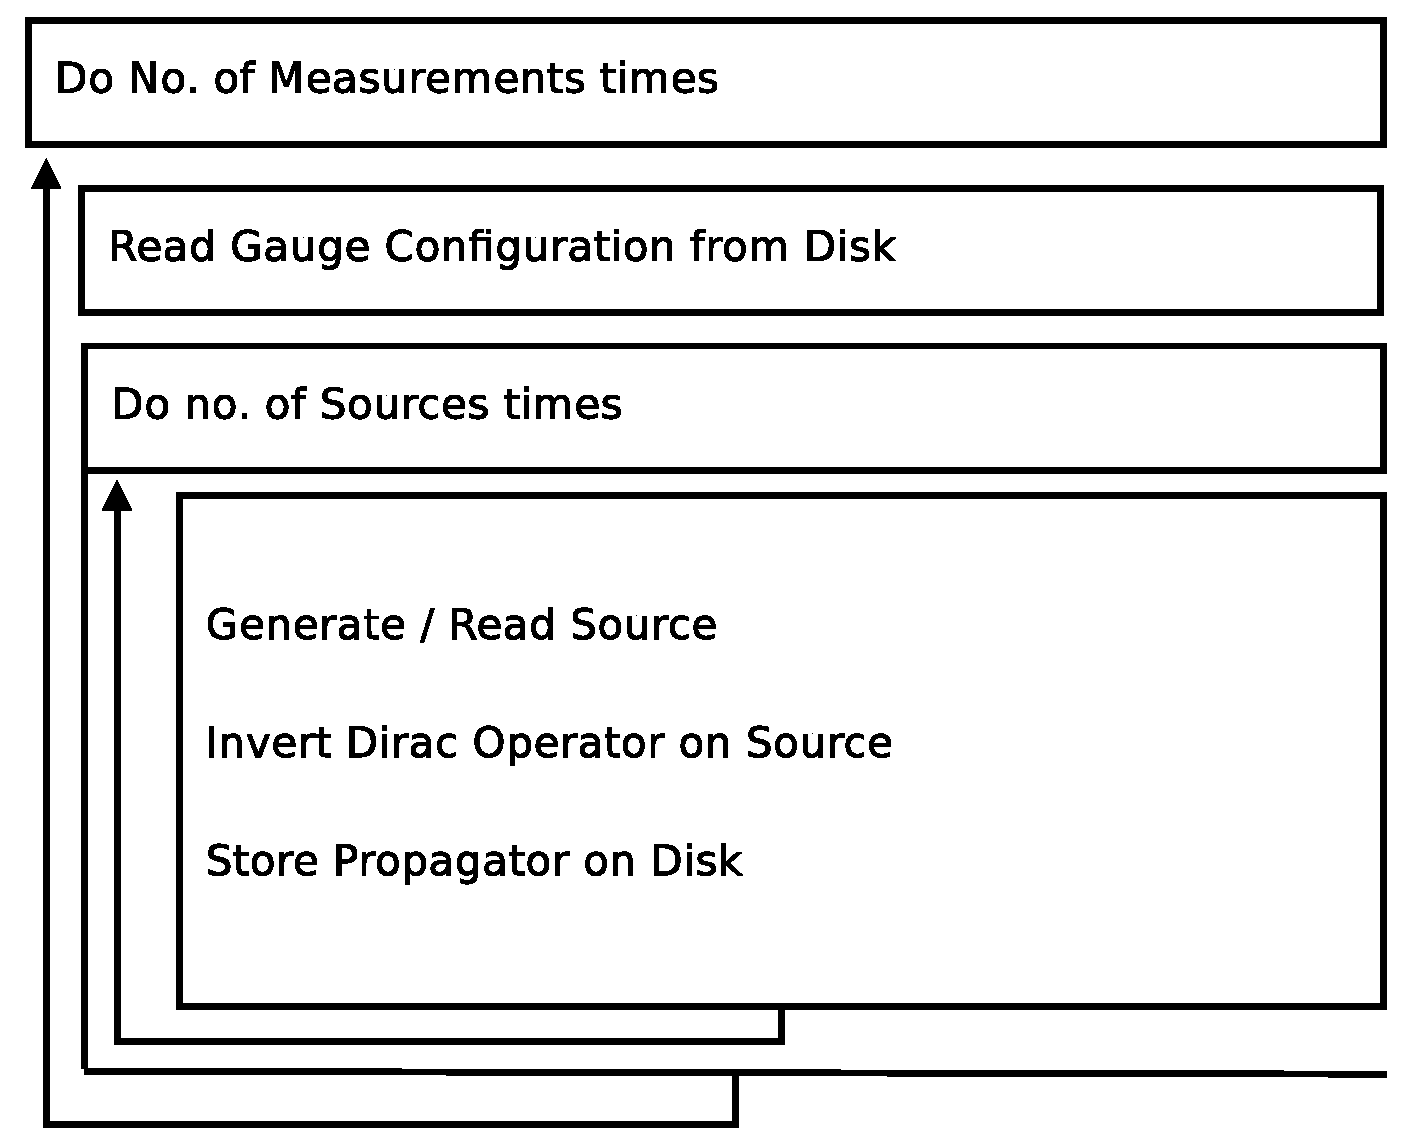
\includegraphics[width=0.7\linewidth]{invertflow.eps}
  \caption{Flowchart for the main part of the {\ttfamily invert} and
    {\ttfamily invert\_doublet} executables.}
  \label{fig:invertflow}
\end{figure}

The two applications {\ttfamily invert} and {\ttfamily
  invert\_doublet} are very similar. The main difference is that in
{\ttfamily invert} the one flavour Wilson twisted mass Dirac operator
is inverted, whereas in {\ttfamily invert\_doublet} the non-degenerate
doublet is inverted. 

The main part of the two executables is depicted in
figure~\ref{fig:invertflow}. Each measurement corresponds to one gauge
configuration that is read from disk into memory. For each of these
gauge configurations a number of inversions will be performed. 

The sources can be either generated or read in from disk. In
the former case the programme can currently generate point sources at
random location in space time. In the latter case the name of the
source file can be specified in the input file. 

The relevant Dirac operator is then inverted on each source and the
result is stored on disk. The inversion can be performed with a number
of inversion algorithms, such as conjugate gradient (CG), BiCGstab,
and others~\cite{saad:2003a}. And optionally even/odd preconditioning
as described previously can be used. 

\subsubsection{command line arguments}

The two programmes offer command line options as follows:
\begin{itemize}
\item {\ttfamily -h|?} prints a help message and exits.
\item {\ttfamily -f} input file name. The default is {\ttfamily
    hmc.input}
\item {\ttfamily -o} the prefix of the output filenames. The default is
  {\ttfamily output}. The code will generate or append to one file
  called {\ttfamily output.para}.
\end{itemize}

\subsubsection{Output}

The program will create a file called {\ttfamily output.data} with
information about the parameters of the run. 
Of course, also the propagators are stored on disc. The corresponding
file names can be influenced via input parameters. The file format
is discussed in some detail in sub-section~\ref{sec:io}.

One particularity of the {\ttfamily invert\_doublet} program is that
the propagators written to disk correspond to the two flavour Dirac
operator of eq.~(\ref{eq:altDh}), i.e.
\[
D_h'(\mu_\sigma,\mu_\delta) = D_\mathrm{W}\cdot 1_f +
i\mu_\sigma\tau^1 + \gamma_5 \mu_\delta \tau^3\, ,
\]
essentially for compatibility reasons. For the two flavour components
written the first is the would be \emph{strange} component and the
second one the would be \emph{charm} one.                             

\subsection{Parallelisation}

The whole lattice can be parallelised in up to 4 space-time directions.
It is controlled with configure switches, see section~\ref{sec:config}.
The Message Passing Interface (MPI, standard version 1.1)  is used to
implement the parallelisation. So for compiling the parallel
executables a working MPI implementation is needed.

Depending on the number of parallelised space-time directions the
$t$-direction, the $t$- and $x$-direction, the $t$-, $x$- and
$y$-direction or the $t$-, $x$- and $y$- and $z$-direction are
parallelised. 

The number of processors per space direction must be specified at run time,
i.e. in the input file. The relevant parameters are {\ttfamily
  NrXProcs}, {\ttfamily NrYProcs} and {\ttfamily NrZProcs}. The number
of processors in time direction is determined by the program
automatically. Note that the extension in any direction must divide by
the number of processors in this direction. 

In case of even/odd preconditioning further constraints have to be
fulfilled: the local number of lattice sites must be even and the
local $L_z$ must be even. Moreover, the local product $L_t\times L_x
\times L_y$ must be even in case of even/odd preconditioning. 


\begin{figure}[htbp]
\centering
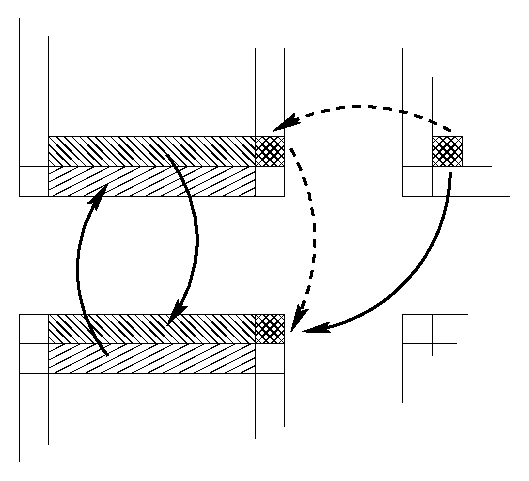
\includegraphics[width=0.65\linewidth]{partition}
\caption{Boundary exchange in a two dimensional parallel setup. One
  can see that the internal boundary is send while the external one
  is received. The corners need a two step procedure.}
\label{fig:partition}
\end{figure}

The communication is organised using boundary buffer, as sketched in
figure~\ref{fig:partition}. 
%In general the order for gauge and spinor fields in memory is as
%follows: first the local fields, then the \emph{right} t-boundary fields, then
%the \emph{left} t-boundary fields, then the \emph{right} x-boundary
%fields, the \emph{left} x-boundary fields and finally the corners (see
%figure \ref{fig:partition}). 
%
The MPI setup is contained in the file {\ttfamily mpi\_init.c}. The
corresponding function must be called at the beginning of a main
program just after the parameters are read in, also in case of a
serial run. In this function also 
the various {\ttfamily MPI\_Datatype}s are constructed needed for the
exchange of the boundary fields. The routines performing the
communication for the various data types are located in files starting
with {\ttfamily xchange\_}.

The communication is implemented using different types of MPI
functions. One implementation uses the {\ttfamily MPI\_Sendrecv}
function to communicate the data. A second one uses non-blocking MPI
functions and a third one persistent MPI calls. See the MPI standard
for details~\cite{mpi:web}. On machines with network capable of
sending in several directions in parallel the non-blocking version is
the most efficient one. The relevant configure switches are {\ttfamily
  --with-nonblockingmpi} and {\ttfamily --with-persistentmpi}, the
latter of which is only available for the Dirac operator with
halfspinor fields, see section~\ref{sec:dirac}.


%%% Local Variables: 
%%% mode: latex
%%% TeX-master: "main"
%%% End: 
